\section{Enfoque Propuesto}

De acuerdo a los requerimientos analizados y en función a los objetivos se propone realizar un sistema modular con arquitectura web que no demande inicialmente un gasto excesivo en infraestructura ni en servicios de terceros, pero que, sin embargo, pueda requerirlos en cualquier momento futuro.

\subsection{Arquitectura e Infraestructura}

Inicialmente, se plantea una arquitectura monolítica, es decir, una aplicación web contenida en un solo repositorio, cumpliendo con el patrón cliente-servidor.

En cuanto a la infraestructura, existen muchas opciones, pero una de las más económicas y que bastará para las etapas iniciales con una cantidad de usuarios no mayor a los 100 activos por día es el shared hosting. Existen también varias ofertas de shared hosting, siendo la más conocida, Hostinger.

Estos servidores brindan paneles de administración intuitivos, además de precios iniciales realmente bajos, pero están limitados a ciertas tecnologías y configuraciones.

\subsection{Stack Tecnológico}

Para lograr la implementación exitosa en el menor tiempo posible, con posibilidad a mejoras futuras, escalabilidad y capacidad de funcionamiento en cualquier servidor, se propone el stack tecnológico TALL (Tailwind, Alpine, Laravel, Livewire). 

\begin{figure}[htbp]
    \centering
    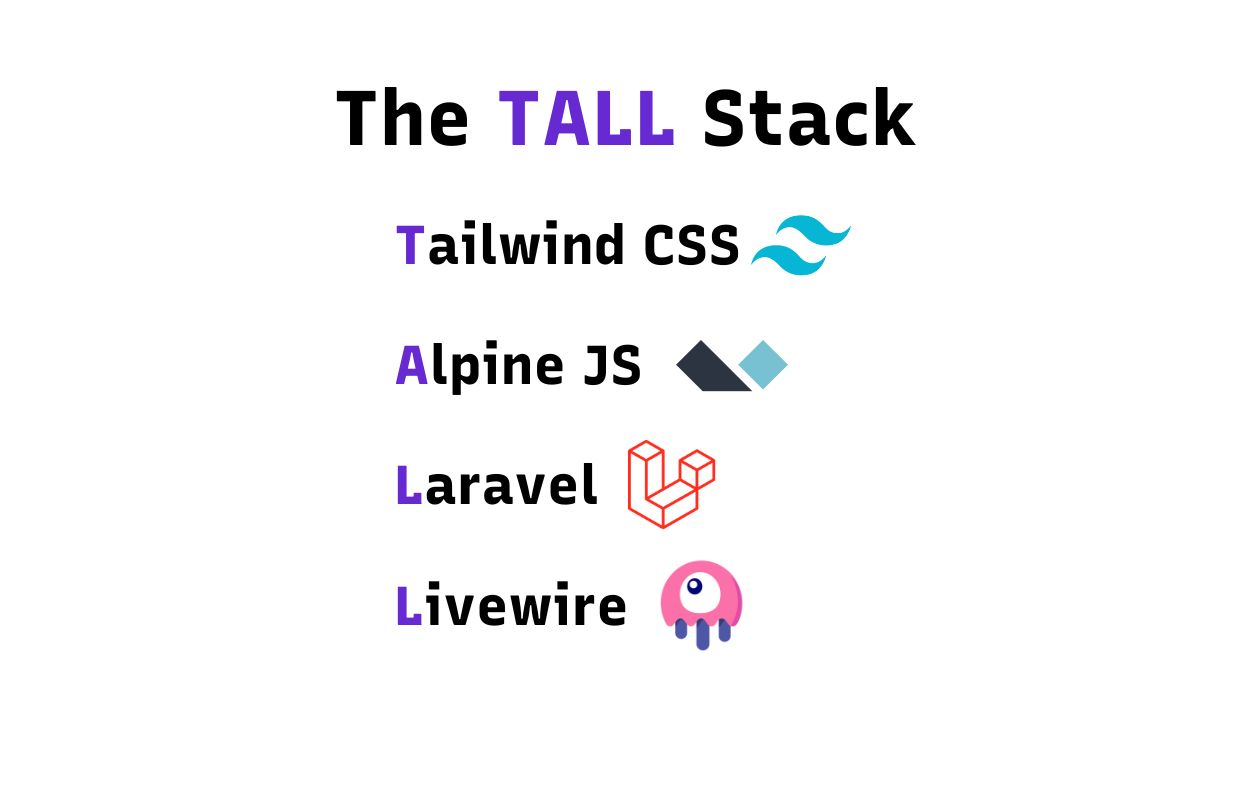
\includegraphics[width=0.7\textwidth]{assets/tall.jpg}
    \caption{Stack TALL}
    \label{fig:tall}
\end{figure}

Además, con el uso de librerías como Filament garantizamos un desarrollo eficiente y a bajos costos, además de versatilidad en caso de desear la creación de un servicio REST API a futuro para aplicaciones móviles e integraciones.

\subsection{División en módulos}

Una buena práctica es poder abstraer el sistema en módulos funcionales independientes. Nuestro análisis nos permitió identificar los siguientes:

\begin{enumerate}
\item Módulo de administración de usuarios,
\item Módulo de reservas y valoraciones (Pieza central),
\item Módulo de administración de anfitrión y registro de datos de hoteles,
\item Módulo de administración general,
\item Módulo de pagos en línea asistidos por humano
\item Módulo de pagos en línea,
\item Módulo de facturación electrónica,
\item Módulo de contabilidad básica,
\end{enumerate}